\section{Approach}
    \label{sec:1}
\subsection{Architecture of the model}
The approach chosen for this problem is based on the training of a CNN. The choice of a CNN was clear, as it is a standard model used in computer vision applications. The architecture of the model was determined by trying out different approaches on the raw data to get a feeling for what works and what should be dismissed. This "trying out" showed, that a high amount of convolutional layers would be needed for the model to work properly. With the amount of data being high, a relatively complex architecture was then chosen for this task, which can be seen in
\autoref{fig:arch}.
\begin{figure}[H]
    \centering
    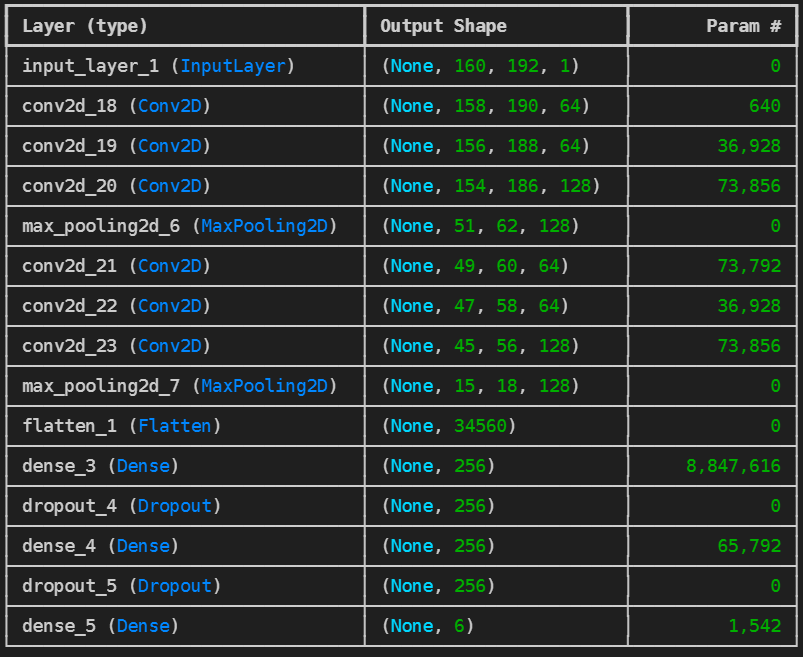
\includegraphics[width=0.7\textwidth]{content/arch.png}
    \caption{Final architecture of the model.}
    \label{fig:arch}
\end{figure}
\noindent
The model consists of two convolutional blocks consisting of 3 convolutional layers and one max-pooling layer respectively. The output of these convolutional blocks is flattened and runs through 2 dense blocks with each one dense layer and one dropout layer.
The number of filters in each block is 64 for the first two convolutional layers and 128 for the last convolutional layer. The kernel size is (3,3) as well as the pool size. 
\subsection{Data preprocessing}
The preprocessing of the data is a crucial step for the success of the chosen method. With the .jpg images being of size (360, 640) and the amount of data being high, down-scaling of the images resolution and size becomes necessary for computation reasons. With this in mind, two methods were implemented, one doing a crop on the image to reduce background, and the other reducing the resolution of the image. 
The initial idea for the cropping was to use a face detection software to dynamically crop each picture according to the drivers face postition. This idea had to be dismissed as the face detection was not as reliable as initially hoped. With many drivers in the "Distraced" class looking to the side or down on their phone, the face detection algorithm started to detect faces in the background of the images, introducing a large bias into the dataset. 
An alternative method was then chosen, which crops 100 pixels from the left and right of every picture, significantly reducing the amount of background for the training of the CNN. A before and after comparison of the cropped images can be seen in \autoref{fig:comp1}
\begin{figure}[H]
    \centering
    \begin{subfigure}{0.48\textwidth}
        \centering
        \adjustbox{valign=c}{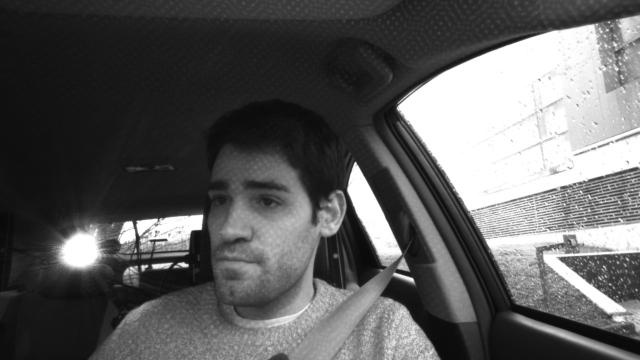
\includegraphics[width = \textwidth]{content/test1.jpg}}
    \end{subfigure}
    \hfill
    \begin{subfigure}{0.48\textwidth}
        \centering
        \adjustbox{valign=c}{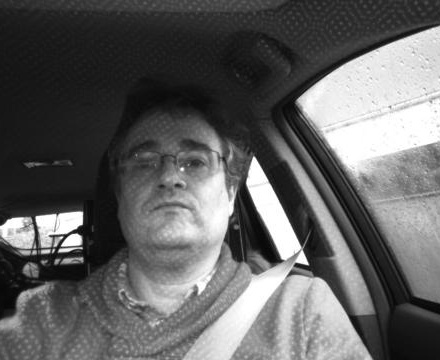
\includegraphics[width = \textwidth]{content/test2.jpg}}
    \end{subfigure}
    \caption{Comparison of the uncropped (left) and cropped (right) images.}
    \label{fig:comp1}
\end{figure}
\noindent
This is possible due to the camera position being relatively consistent throughout all images. A greater crop sometimes led to the faces or class relevant objects being cropped off and was thus not implemented. 
The cropped images were then scaled down to a resolution of 192 $\times$ 160 using the OpenCV \cite{opencv} library.
\section{Data augmentation and overfitting optimization}
    \label{sec:2}
This section will present the precautions taken to compensate for possible overfitting of the data and the data augmentation done to balance the amount of classes in the dataset.
\subsection{Data augmentation}
Classes like "Yawn" or "Drinking" have very few entry in contrast to the rest of the dataset, with relative amounts to the total dataset size being 
Safe driving: $41.59\%$,
Dangerous driving: $31.25\%$,
Distraced: $14.00\%$,
Sleepy driving: $6.59\%$,
Yawn: $3.68\%$,
Drinking: $2.89\%$ .
For this reason data augmentation is implemented to account for the drastic class imbalances.
The original approach for the augmentation process was to generate augmented data to fill up all classes to the number of entries of the largest class. This resulted in an immense amount of data being generated which could not be handled by the computational power avaiable. An alternative approach was then chosen, in which all classes are scaled to 2000 entries. This resulted in cutting off entries from the top three largest classes and only a minimal amount of data augmentation in the three smallest classes. 
The augmentation was conducted using the tensorflow.keras.preprocessing.image.ImageDataGenerator method, alongside a self implemented noise generator. The ImageDataGenerator does a random augmentation for each image based on initially set parameters. The augmentations applied to the images are rotations up to 40 degrees, shifts in width and height up to a value of 0.2, shear and zoom up to a value of 0.3 and a possible vertical flip of the image. 
\section{Results and comparison to alternative Method}
    \label{sec:3}